%\newcommand{\Cerenkov}{\v{C}herenkov~}

A charged particle travelling faster
than the speed of light in the medium will create an electromagnetic
disturbance in the medium. The radiation emitted by this process is
called \Cerenkov\ radiation after its discoverer.

\Cerenkov\ radiation is conically distributed about the trajectory of the
particle, with an angle given by
$$
	\cos{\theta} = \frac{1}{\beta n}
$$
where the index of refraction $n = c/u$ and $\beta = v/c$, with $c$
the speed of light in vacuum, $u$ the speed of light in the medium,
and $v$ the speed of the particle.

The index of refraction allows one to control the threshold particle velocity 
$v_{T}=u=c/n$ below which there is no \Cerenkov\ light produced, and above which there 
is \Cerenkov\ light produced.  For a gas, the quantity $n-1$ is proportional to the pressure, 
so adjusting the pressure of the gas allows one to select the
threshold velocity. Adjusting the threshold velocity then allows one to select particles of
different mass.  Given the same momentum, two particles of different mass
will have different velocity.  Therefore, a \Cerenkov\ detector can be tuned,
for instance, to distinguish electrons from pions.



The SHMS \Cerenkov\ detector consists of a large cylindrical tank,
with outer flange radius of 1.88~m or 74 inch, and bolt to bolt length
of 1.3~m or 51.1 inch. The detector contains four mirrors which focus
light onto four 5 inch Hamamatsu R1584 photo multiplier tubes (PMT's),
as shown in Fig~\ref{fig:hgc}.


The main detector cylinder is made of a 0.5 inch thick T6061-T6
Aluminum sheet with radius of 1.725~m or 67.9~inch. Both circular ends
have been covered with 0.04 inch thick 2024-T4 Aluminum windows. These
windows were hydrostatically formed (and hence tested) at a pressure
of 45 PSI.In addition, the windows were hydrostatically tested at a
pressure of 60 PSI. The tank itself was helium leak checked and is
leak free on a scale of 10$^{-8}$ Atm-cm$^3$/s. HGC detector
configuration only allows sub atmospheric pressure operation, thus
under no circumstance the detector pressure shall exceed 1 Atm. Each
of the aluminum windows are sandwiched between the detector vessel and
a thick aluminum flange. All three components are clamped with
stainless steel bolts with washers and silicon bronze
nuts. Installation torque for each bolt is specified to be 26
lb$\cdot$ft.

%Detailed information on this testing program can be found in \cite {bi:tank}, \cite {bi:wind}.
% 
% \subsection{PMT}
% 
% PMT is not located inside of the vessel inclosure!
% 
% 
% PMT required negative voltage ! 
% 
% Discharge
% 
% 






%	The HMS Cerenkov detector consists of a large cylindrical
%tank, $\phi_{in} = 59"$, $L = 60"$, containing two mirrors which focus
%light onto two 5 inch Burle 8854 multiplier photo  tubes (PMT's). The tank
%has been installed with 0.04 inch thick 2024-T3 Aluminum windows
%covering the circular ends of the cylindrical tank. These
%windows were hydrostatically formed (and hence tested) at a pressure
%of 28 PSI. The tank itself was helium leak checked and is leak free
%on a scale of 10$^{-8}$ Atm-cm$^3$/s. In addition, the tank was hydrostatically
%tested at a pressure of 35 PSI. Detailed information on this testing
%program can be found in \cite {bi:tank}, \cite {bi:wind}.


\begin{figure}[ht]
\centering
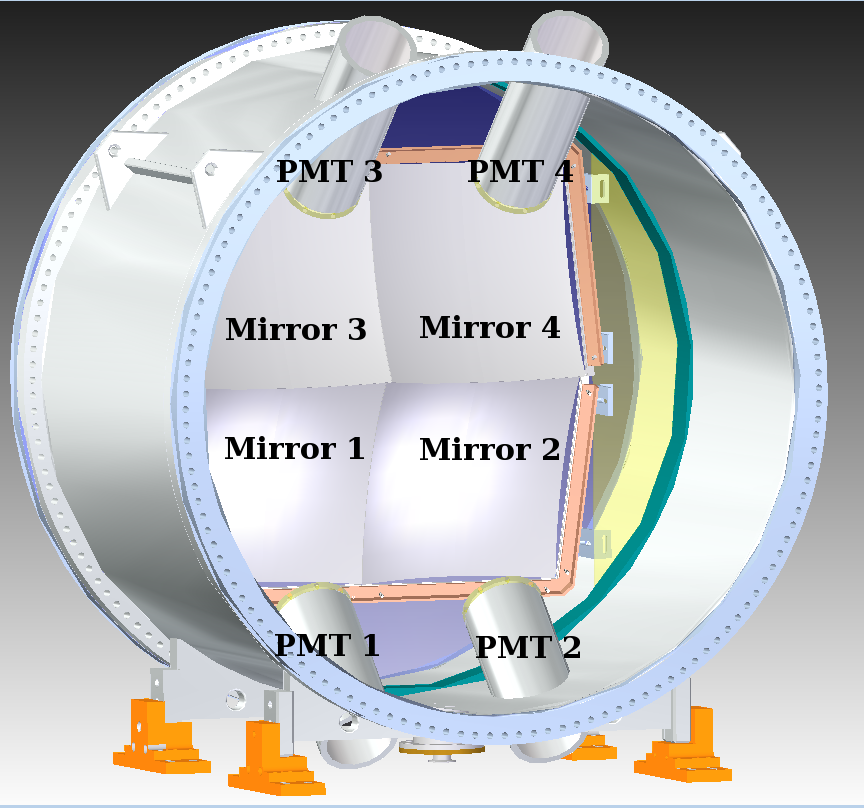
\includegraphics[width=0.75\linewidth]{cherenkov_front}
\caption{CAD Drawing of SHMS HGC detector. \label{fig:hgc}}
\end{figure}



The HGC tank is mounted on the detector rails using a three point
alignment scheme. The rails are easily capable of supporting the
weight of the tank without deformation. The gas handling system for
the tank is designed to enable the tank to be filled with pure gas,
C4F10 or CO2, at the desired operating pressure which is 0.2-1
Atm. Detector operating pressure must not exceed 1 Atm.

{ \color{red}  

The system consists of a filled gas bottle and primary pressure
regulator which are in a bottle rack that is welded to the bottom of
the SHMS detector hut on the small angle side at a height of about six
inches from the hall floor. The primary regulator is a Matheson model
2596 with a maximum outlet pressure of 400 PSI.  During fills this
regulator should be set to 150 PSI. The outlet of this pressure
regulator is connected to the main gas control panel which is mounted
on the first floor balcony of the detector hut behind the dipole
control racks. All connecting tubes in the system are 0.25 inch
diameter stainless steel tubing with the exception of the nitrogen
purge line which is thick wall tygon. At the entrance to the gas panel
there is a 0-300 PSI gauge so that the pressure in the inlet line can
be viewed by the operator.


The line is then relieved by a Circle Seal relief valve set at 200 PSI.
After this, the gas passes through a second regulator (Matheson 3420)
which has an outlet pressure range of 0-60 PSI. This regulator can be set at
up to 40 PSI for high flow during the early stages of fills
(the line is relieved further downstream by a second
Circle Seal relief valve set at 45 PSI) and then reduced as
the desired operating pressure is approached. Following the second regulator
and its relief valve the gas passes through oil and oxygen filters.
A 120 Volt AC solenoid valve (ASCO) switched with a solid state
relay is used to isolate the gas flow from the tank. The state of
the relay and hence the valve is indicated by a LED on the panel.
The gas line is routed through an opening in the floor of the detector hut
to the tank inlet. A gauge on the panel allows the operator to view
the pressure in the inlet line (the same as the tank pressure
when the subsequent manual valve is open, see following).
At the inlet there is a pair of manual valves (NUPRO)
which allow the fill line to be purged.
During operation the valve which vents the
line to atmosphere is closed and the valve to the tank inlet is open.
The tank is relieved by a 1 inch diameter, 1 PSI pop off (NUPRO) which was
sized to take the
maximum flow of the second regulator even if that regulator has failed
wide open. There is a pressure gauge on the tank so that its condition
can be determined by workers in the shield house. In addition,
there is a Omega pressure transducer (PX-305-05A) and a temperature
transducer attached to the tank. These are read out and powered by
units (Omega) which are located below the gas panel.  Outputs of these
are currently viewed with a video camera attached
to a monitor in the counting house.

Before filling, the tank is first cleaned by executing several pump
and purge cycles. The pump that is used to evacuate the tank is located on a
platform welded to the small angle side of the shield house balcony
which can be accessed from the small angle side of the SHMS carriage.
Eventually, it will be possible to switch the power for this pump
from the gas control panel with a relay but currently it
is necessary to turn the pump on and off with a switch located on the pump.
The low pressure side of this pump is equipped with a liquid nitrogen
cold trap to prevent any contamination of the tank (or mirrors !)
with pump oil. This trap will remain filled for approximately
12 hours and should always be checked before use. There is currently
a manual valve located at the \Cerenkov\ tank that isolates the tank from
the pump.  This valve will later be replaced by a pneumatically actuated
solenoid valve that will be controlled from the gas panel.
There is a manual valve on the tank which is equipped with a hose
barb through which clean nitrogen purge gas can be admitted to the tank.
The nitrogen gas comes from a spigot on the SHMS cryogenic handling system
located along the upper catwalk of the SHMS. The nitrogen system
delivers gas at a line pressure of $\approx$ 40 PSI (this pressure can
be read on a gauge at the pivot end of the catwalk). The flow
rate is readable from a flow meter attached to the spigot. A flow of
about 150 - 200 cfm is reasonable. The tank should not be filled to
more than -5 in Hg during purge cycles.

}



The tank is a confined space and hence this activity represents an ODH
hazard. Stickers indicating this have been placed on the PMT
ports. Before an entry into the tank the atmosphere in the interior
must be surveyed by a member of the physics division EH$\&$S staff.

The mirrors in the HGC may require adjustment for optimal focusing on
the PMT faces. Small adjustment to the mirror position cannot be done
while the detector is mounted. The adjustment to mirror position can
only be performed when the detector vessel is in the horizontal
position with both aluminum windows completely removed. While the HGC
is mounted, up to 1~cm adjustment to PMT position can be made by
repositioning the plastic eccentric PMT holders. This adjustment
should only be done by personnel who completely understand the design
of the PMT mounting assembly.

%The interior of the tank has foot braces and welded hand holds which allow this work at the angle of the detector rails.





\paragraph{PMTs} From Fig~\ref{fig:hgc}, there are four aluminum sleeves welded onto
the detector cylinder, where each sleeve hosts one PMT assembly. Note
that the PMT assembly is outside of the vessel enclosure, viewing
the \Cerenkov\ radiation through a quartz viewport. The inner end of
each sleeve is installed with a quartz window that provides vacuum
seal. Hamamatsu R1584 PMT assembly to which is glued a custom
flat-head quartz adapter. The PMT and quartz adapter is pressed
against the viewport, held in position via spring pressure. The
contacting optical surfaces are coupled with a thin layer of
UV-transparent silicon grease. A spring lock-in mechanism (open end of
the sleeve) is used to provide mechanical pressure to ensure good
contact between optical surfaces; and a customized rubber cone is used
to provide light seal.

% R1584 PMT assembly with a flat-head quartz adapter is pressed against the window, the contacting optical surfaces are coupled with a thin layer of UV transparent silicon grease; 

\begin{table}[t]
\centering
  \begin{tabular}{ |c | c | c |} \hline PMT \# & Serial \# &
    Voltage \\ \hline 1 & LA0274 & 2132 \\ \hline 2 & LA0272 &
    1967 \\ \hline 3 & LA0273 & 1926 \\ \hline 4 & LA0271 &
    2013 \\ \hline \end{tabular} \caption{Serial number and initial
    recommended operating voltage for each PMT.}  \label{tab:hgc_volt}
\end{table}

   

The SHMS HGC 5 inch PMTs use {\bf negative} HV. The PMT photo-cathode
is powered at hazardous high negative voltage and the mu-metal shield
is grounded, so there is a ~2000V potential difference between the PMT
and the shield. Note that the Aerogel and Nobal Gas \Cerenkov\
detectors use PMT bases that are designed for positive HV, therefore
one must only use labelled HV cables for HGC. The HV is supplied by
one pod of the {\em CAEN} power supply. The safe PMTs operating
voltages are between 1500 and 2400 Volts. For the initial
commissioning stage, the operation voltages should not exceed 2200
Volts. The serial number and initial recommended operating voltages
for each PMT are listed in Table~\ref{tab:hgc_volt}. At the
recommended voltage, the expected average pulse height for a PMT
signal should be $\sim$400~mV and rates $\sim$100~Hz.


%at the time of installation we did extensive tests and confirmed no discharge.  Then we can explain what might happen if there is a future breakdown of electrical insulation and what to look for. 

Fig~\ref{hgc:goodsignal} shows an example of regular signal from a
R1584 PMT; Fig~\ref{hgc:discharge} shows an example of discharging
signal indicating a breach of electrical insulation between the
photo-cathode and mu-metal shield. The discharging signals have very
distinctive characteristics since they are relatively large pulses
($>$5 Volts) that are $>$100~ns long.

At the time of installation, extensive tests were performed for all
four PMTs and confirmed no discharge at 2000 Volts. Once discharging
signal is observed, one should carefully monitor the rate as well as
report the incidence immediately. The primary suspect for causing
discharge puilse is a possible electric insulation breach between the
photo tube and mu-metal shield. Further diagnose would require
complete removal of the PMT assembly from the aluminum sleeve while
all four PMTs are switched off. Electric insulation that covers the
inner edge of mu-metal shield cylinder must be carefully
inspected. Once the location of discharge is identified, it is
recommended to seal the suspect area with few layers kapton tape.







\begin{figure}
     \centering
     \subfloat[][Regular Signal]{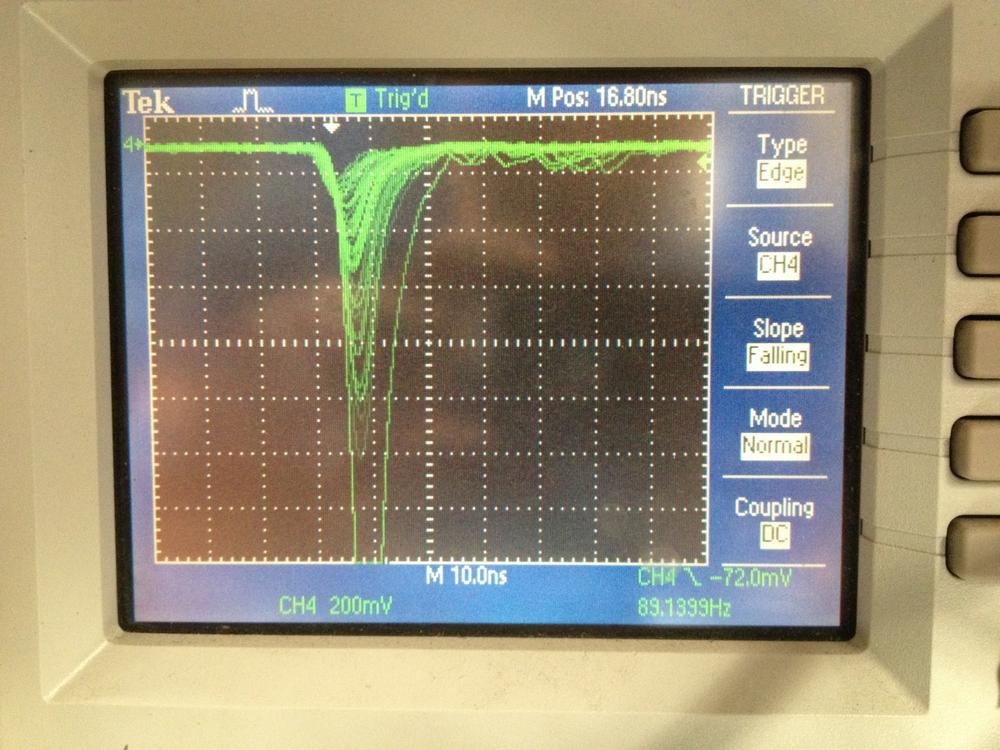
\includegraphics[width=0.45\linewidth]{pmt4_1047}\label{hgc:goodsignal}}~
     \subfloat[][Discharge]{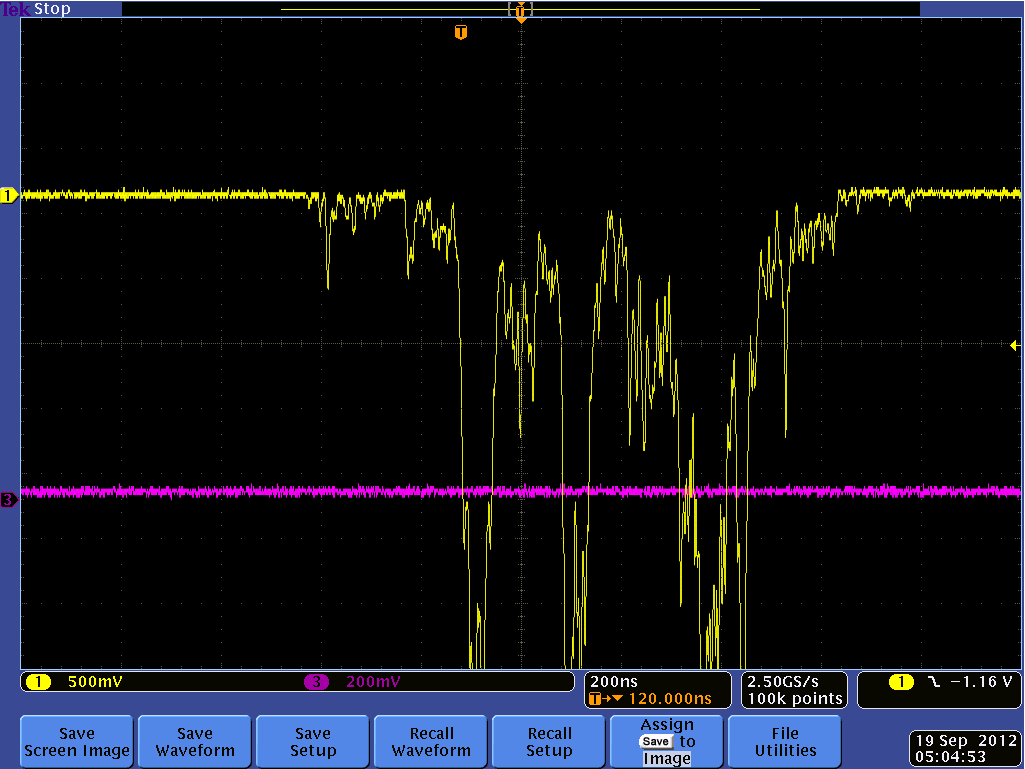
\includegraphics[width=0.45\linewidth]{discharge}\label{hgc:discharge}}
     \caption{(a) shows example of regular PMT signal; (b) shows a discharged signal.}
     \label{hgc:signal}
\end{figure}


% 
% PMT serial number: LA0274, LA0272, LA0273, LA0271
% 
% Initial recommanded voltage: 2132, 1967, 1926, 2013 Volts.
% 






{\color{red}


\paragraph{Operation Procedures}
% 
% \begin{figure}
% %\GHS
% 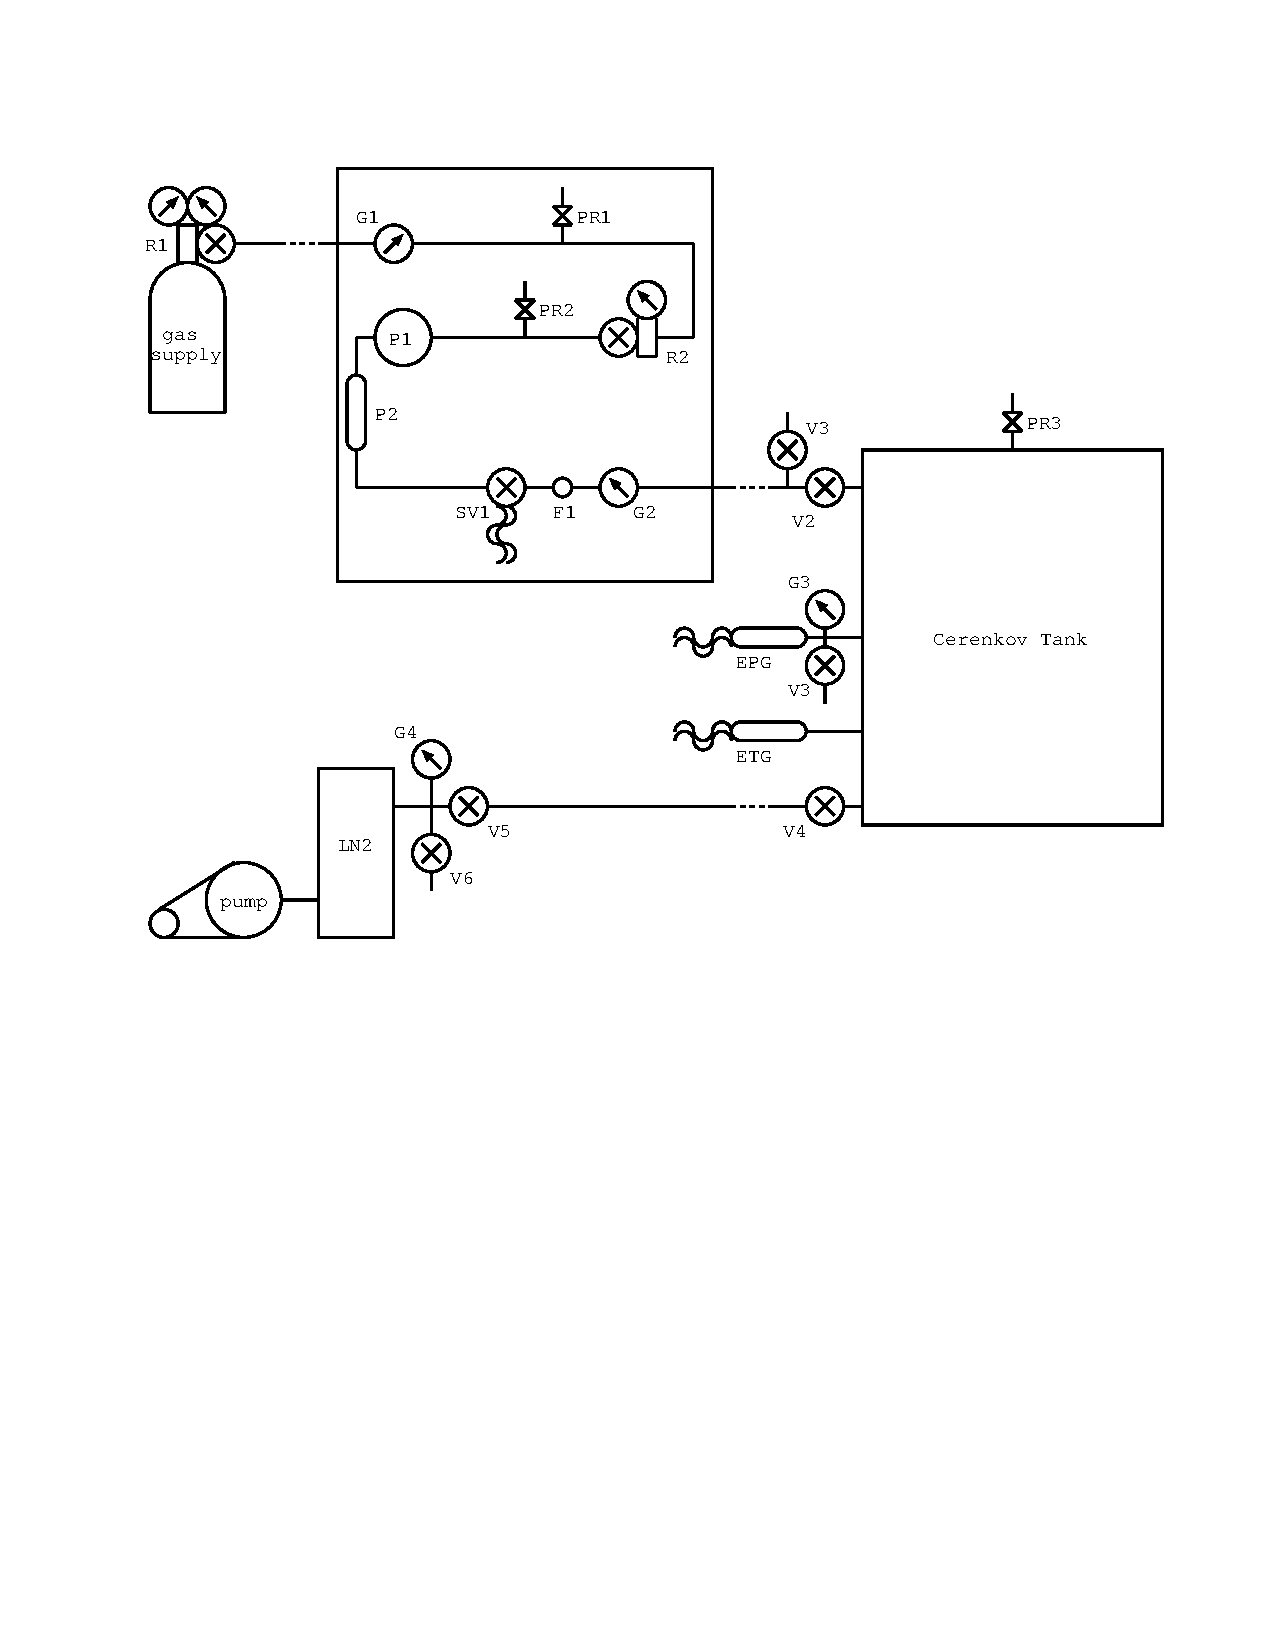
\includegraphics[height=5in,width=6in]{HMSgasC.pdf}
% \caption{The Gas Handling System for the HMS \Cerenkov\ Detector. \label{fig:gas}}
% \end{figure}
% 
The SHMS \Cerenkov\ Detector operates either as an $\pi$/$\kappa$ e/$\pi$ or
discriminator. Each mode has a unique set of procedures to prepare the tank
for operation. 


% The nomenclature used in the description of these operation procedures refers to Figure~\ref{fig:gas}, showing the system of gas handling.The components shown inside the dashed box of Figure~\ref{fig:gas}, are all located on the Gas Control Panel.

\paragraph{$\bf{\pi}$/$\kappa$ Procedures}
This mode of operation typically requires the tank to be filled with
C4F10 at pressures varying from 0.2 to 1~Atm. The detector is pumped
down to ~1 milli-torr, then refilled with C4F10 gas.

Because the operating pressure is slightly subatmospheric, a pump and fill
procedure is employed.  First make sure that:
\begin{itemize}
%\item The 40~mil windows are installed and oriented such that they curve towards the interior of the tank.
\item Valves {\bf V1-V6} are closed.
\item The LN2 trap is filled.
\item There is enough oil in the pump.
\end{itemize}
The tank is now ready to be evacuated.
\begin{itemize}
\item Turn on the pump.
\item Slowly open {\bf V5}.  This evacuates the pump line.
\item Open very slowly {\bf V4}.  Since this valve connects the pump line to
the detector volume, the pump will work very hard.  Meter this valve
so that the pump is never under extreme stress.  It will take approximately
20~minutes to pump down the tank.
\end{itemize}
The tank can now be filled.
\begin{itemize}
\item Locate the boiloff manifold on the walkway on the top level of the
spectrometer, at the gap between Q3 and the dipole.
\item Turn the valve on this manifold open slightly so that the flow meter
barely registers a flow.
\item Connect the remaining end of the Tygon tubing to the vent of valve
{\bf V3} with a hose clamp.
\item Open valve {\bf V3}.
\item Increase the flow on the flow meter.  Do not exceed 100~cfpm.
\item When {\bf G3} or {\bf EPG} reach the operating pressure, close
the manifold valve.
\item Close {\bf V3}.
\end{itemize}
The fill should take approximately 30 minutes.  The detector should
NEVER be left unattended during a fill.  Frequently check the pressure
in the tank and be aware when the pressure is near to one atmosphere.
DO NOT let the pressure exceed one atmosphere under any circumstances;
doing so risks damage to all of the equipment and personnel in the
detector hut.  This pump/fill procedure is usually repeated at least
once to ensure the purity of the gas.






%  Because these operating pressures are

% 
% 
%  Because these operating pressures are
% greater than 1~atm, the detector must be filled by dilution.  Contamination
% from air, however, is not a major problem as the optical absorption properties
% of air are actually more favorable than those of Freon-12 itself; the only
% difficulty is the increase in pressure needed for a mixture of air and Freon
% to achieve the same pion momentum threshold as for a pure sample of Freon.
% 
% First prepare the gas handling system:
% \begin{itemize}
% \item Make sure that the 60~mil windows are installed and oriented such that
% they bulge outwards from interior of the tank.
% \item Close the valves {\bf V2-V4}, and the valve on regulator {\bf R1}.
% {\bf V1}, {\bf SV1}, and the valve on regulator {\bf R2} should be
% open.
% \item Open the valve on the gas supply bottle.
% \item Adjust {\bf R1} to approximately 60 psig.
% \item Open the valve on {\bf R1}.
% \item Check to make sure gauge {\bf G1} agrees with the pressure setting
% on {\bf R1}.
% \item Adjust {\bf R2} so that a small flow is detected out the vent of
% {\bf V1}.
% \item Close {\bf V1}.
% \item Adjust {\bf R2} to regulate at the required operating pressure.
% \end{itemize}
% The tank is now ready for the dilution process.  These steps should be
% repeated as few times as possible to minimize the quantity of Freon-12 emitted
% to the atmosphere.
% \begin{itemize}
% \item Record the tank pressure.
% \item Open valve {\bf V2}.
% \item Monitor the gas pressure until it reaches the required operating pressure.
% NEVER let the pressure in the detector exceed 3~atmospheres.
% \item Record the final pressure.
% \item Open {\bf V3} to vent the tank.
% \end{itemize}
% From the recorded pressure readings, the threshold momentum of the mixture
% of air and Freon-12 can be calculated (assuming the volume of the tank is
% fixed).
% 




\paragraph{$e$/$\bf{\pi}$ Procedures}
The procedure for $e$/$\bf{\pi}$ separation runs with 0.2 to
1 atmospheres of C4F10.  This is just a small modification to the
current $\pi$/$\kappa$ procedures.


% $e$/$\bf{\pi}$ running can also be accomplished using a Nitrogen fill.
% This mode of operation requires the tank to be filled with approximately
% 13.5~psia of $\rm{N_2}$. The boiloff from the spectrometer magnets is a
% perfect source of clean, dry Nitrogen, and is normally used to fill the
% \Cerenkov\ tank.

 
Because the operating pressure is slightly subatmospheric, a pump and fill
procedure is employed.  First make sure that:
\begin{itemize}
%\item The 40~mil windows are installed and oriented such that they curve towards the interior of the tank.
\item Valves {\bf V1-V6} are closed.
\item The LN2 trap is filled.
\item There is enough oil in the pump.
\end{itemize}
The tank is now ready to be evacuated.
\begin{itemize}
\item Turn on the pump.
\item Slowly open {\bf V5}.  This evacuates the pump line.
\item Open very slowly {\bf V4}.  Since this valve connects the pump line to
the detector volume, the pump will work very hard.  Meter this valve
so that the pump is never under extreme stress.  It will take approximately
20~minutes to pump down the tank.
\end{itemize}
The tank can now be filled.
\begin{itemize}
\item Locate the boiloff manifold on the walkway on the top level of the
spectrometer, at the gap between Q3 and the dipole.
\item Turn the valve on this manifold open slightly so that the flow meter
barely registers a flow.
\item Connect the remaining end of the Tygon tubing to the vent of valve
{\bf V3} with a hose clamp.
\item Open valve {\bf V3}.
\item Increase the flow on the flow meter.  Do not exceed 100~cfpm.
\item When {\bf G3} or {\bf EPG} reach the operating pressure, close
the manifold valve.
\item Close {\bf V3}.
\end{itemize}
The fill should take approximately 30 minutes.  The detector should NEVER
be left unattended during a fill.  Frequently check the pressure in the tank
and be aware when the pressure is near to one atmosphere.  DO NOT let the pressure
exceed one atmosphere under any circumstances; doing so risks damage to all of
the equipment and personnel in the detector hut.  This pump/fill procedure is usually 
repeated at least once to ensure the purity of the gas.

}


